\documentclass[11pt]{article}

\usepackage{fancyhdr}
\pagestyle{fancy}
\newcommand\course{ASTR 102}
\newcommand\hwnumber{5}
\newcommand\duedate{November 24, 2020}

\lhead{Oliver Tonnesen\\V00885732}
\chead{\textbf{\Large Lab \hwnumber{} Report}}
\rhead{\course\\\duedate}

\usepackage[
	backend=biber,
	url=true
]{biblatex}
\addbibresource{lab5.bib}
\usepackage{enumitem}
\usepackage{graphicx}
\usepackage{url}
\usepackage{pgfplots}
\usepgfplotslibrary{units}
\pgfplotsset{width=10cm,compat=1.9}

\usepackage{pdflscape}

\usepackage{float}

\usepackage{array}
\newcolumntype{L}{>{\centering\arraybackslash}m{2.5cm}}

\usepackage{amsmath,amsfonts,amssymb}
\DeclareMathOperator{\ly}{ly}
\DeclareMathOperator{\pc}{pc}
\DeclareMathOperator{\yr}{yr}

\usepackage{listings}
\lstset{language=Python,
breaklines=true,
keywordstyle=\color{blue},
identifierstyle=\color{black},
stringstyle=\color{mylilas},
commentstyle=\color{mygreen},
showstringspaces=false,
numbers=left,
numberstyle={\small \color{black}},
numbersep=9pt,
emph=[1]{for,end,break},
emphstyle=[1]\color{red}
}


\begin{document}
\section{Objective}
In this lab, we repeat Edwin Hubble's experiment that lead to his discovery of the Universe's expansion.


\section{Introduction}
In this lab we use observations of supernovae to estimate the velocity at which distant galaxies travel, and in turn to estimate the size and age of the Universe.
Using known wavelengths of spectral lines, we calculate the redshifts of distant galaxies to estimate their recessional velocities.
Using these galaxies' velocities, we can estimate the size of the observable Universe, along with the age of the entire Universe.



\section{Procedure}
Using \cite{WISeREP}, we obtained observations of ten recent supernovae.
Since we know the Si II absorption line should be lie at $\lambda = 6\;150\;\textrm{\r{A}}$, we determined the redshift of each supernova by taking the difference of this wavelength with the observed wavelength of the Si II absorption line.
We found the apparent magnitudes of these ten supernovae using \cite{supernovacatalog}.

After doing this for all ten supernovae, we did a series of calculations (seen in Section~\ref{calculations}) to derive the recessional speed and distance from Earth of each of the galaxies containing the ten supernovae.
We plotted these points and found the line of best fit passing through them.
The slope of this line is our estimate for $H_0$, Hubble's constant.

Using Hubble's constant, we derived further properties relating to these galaxies and to the Universe as a whole.


\section{Observations, Tables, and Graphs}
\begin{landscape}
\clearpage
\thispagestyle{empty}
\begin{table}[H]
\caption{Hubble Redshift Distance Relation.}
\begin{center}
\def\arraystretch{1.5}
\begin{tabular}{| L | L | L | L | L | L | L |}
	\hline
	IAU name & Observed wavelength & Wavelength Difference & Recessional Speed & Apparent magnitude & Distance modulus & Distance \\ \hline
	-- & $\lambda'$ & $(\lambda' - \lambda)$ & $v$ & $m$ & $\mu$ & $D$ \\ \hline
	-- & [\r{A}] & [\r{A}] & [km/s] & [mag] & [mag] & [Mpc] \\ \hline
	\hline
	SN 2017gah & 6204.73 & 54.73 & 2669 & 15.60 & 34.60 & 83.17 \\ \hline
	SN 2018aoz & 6185.67 & 35.67 & 1740 & 12.25 & 31.25 & 17.78 \\ \hline
	SN 2018hdo & 6402.15 & 252.15 & 12300 & 17.40 & 36.40 & 190.5 \\ \hline
	SN 2018hpu & 6562.05 & 412.05 & 20100 & 17.40 & 36.40 & 190.5 \\ \hline
	SN 2018hss & 6414.45 & 264.45 & 12900 & 17.90 & 36.90 & 239.9 \\ \hline
	SN 2018jky & 6239.66 & 89.66 & 4373 & 15.33 & 34.33 & 73.45 \\ \hline
	SN 2019tja & 6215.32 & 65.32 & 3186 & 14.70 & 33.70 & 54.95 \\ \hline
	SN 2019vju & 6229.17 & 79.17 & 3861 & 16.17 & 35.17 & 108.1 \\ \hline
	SN 2020tld & 6218.89 & 68.89 & 3360 & 15.98 & 34.98 & 99.08 \\ \hline
	SN 2020xyw & 6216.51 & 66.51 & 3244 & 16.52 & 35.52 & 127.1 \\
	\hline
\end{tabular}
\end{center}
\label{table:redshift-distance}
\end{table}
\clearpage
\end{landscape}

\begin{figure}
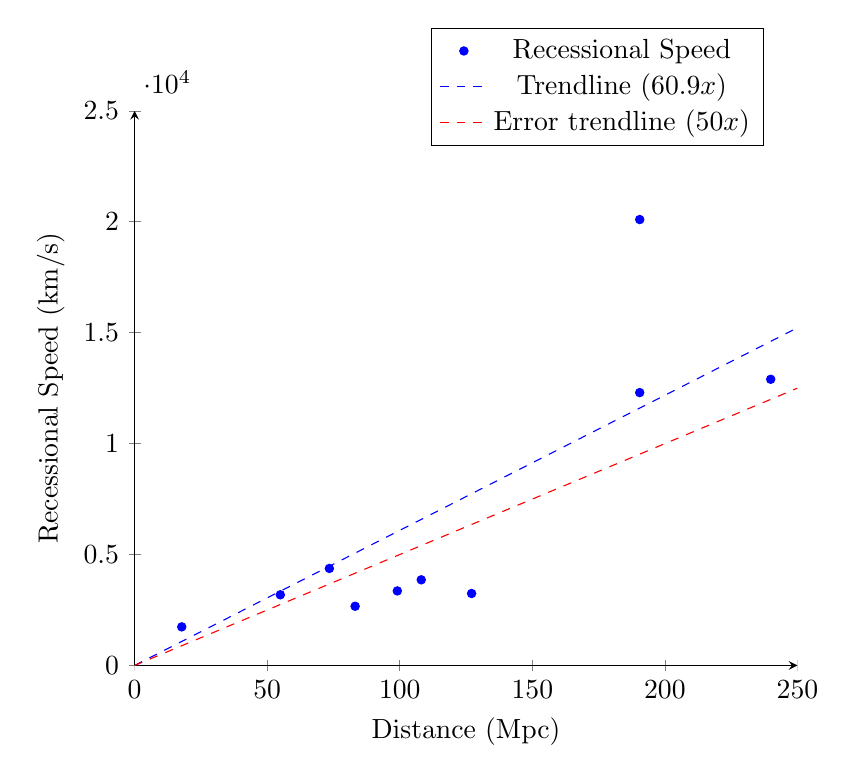
\begin{tikzpicture}
	\begin{axis}[
		axis lines=left,
		xlabel={Distance (Mpc)},
		ylabel={Recessional Speed (km/s)},
		xmin=0, xmax=250,
		ymin=0, ymax=25000,
		legend style={
			at={(0.95,1.15)},
		},
	]
	\addplot [
		only marks,
		mark size=1.5pt,
		color=blue,
	] coordinates {(83.17,2669) (17.78,1740) (190.5,12300) (190.5,20100) (239.9,12900) (73.45,4373) (54.95,3186) (108.1,3861) (99.08,3360) (127.1,3244)};
	\addlegendentry{Recessional Speed}
	\addplot [
		domain=0:250,
		style=dashed,
		color=blue,
	] {60.9*x};
	\addlegendentry{Trendline ($60.9x$)}
	\addplot [
		domain=0:250,
		style=dashed,
		color=red,
	] {50*x};
	\addlegendentry{Error trendline ($50x$)}
	\end{axis}
\end{tikzpicture}
\caption{Recessional Speed vs. Distance of 10 supernovae. See columns 4 and 7 of Table~\ref{table:redshift-distance}.}
\label{graph:speedvdistance}
\end{figure}


\section{Calculations} \label{calculations}
For all following calculations regarding values in Table~\ref{table:redshift-distance}, we will use the supernova SN 2020xyw as an example.

\subsection*{Recessional speed given wavelength difference $\Delta\lambda$}
\[v = c \frac{\Delta\lambda}{\lambda} = 300\;000\;\textrm{km/s} \cdot \frac{66.51\;\textrm{\r{A}}}{6150\;\textrm{\r{A}}} = 3 244\;\textrm{km/s}\]

\subsection*{Distance modulus given apparent magnitude}
Recall that we assume all supernovae to have a constant absolute magnitude of $M = -19.0$.

\[\mu = m - M = 16.52 - 19.0 = 35.5\]

\subsection*{Distance given distance modulus}
\[D = 10^\frac{\mu - 25}{5} = 10^\frac{35.5 - 25}{5} = 127.1\;\textrm{Mpc}\]

\subsection*{Distance to edge of Universe}
The distance at which the velocity of a galaxy will be equal to the speed of light is the value of $x$ for which $y = 300\;000$ in the equation $y = H_0x$; in other words, $x = \frac{c}{H_0}$.

\[\frac{c}{H_0} = \frac{300\;000\;\textrm{km/s}}{60.9\;\frac{\textrm{km/s}}{\textrm{Mpc}}} = 4\;922\;\textrm{Mpc}\]

\[4\;922\;\textrm{Mpc} \cdot \frac{3.26\;\textrm{ly}}{1\;\textrm{Mpc}} = 16\;048\;\textrm{Mly}\]

\[16\;048\;\textrm{Mly} \cdot \frac{1\;000\;\textrm{Mly}}{1\;\textrm{Gly}} = 16.04\;\textrm{Gly}\]

\subsection*{Age of Universe given Hubble's constant $H_0$}
\[\frac{1\;000\;\frac{\textrm{Gy $\cdot$ km/s}}{\textrm{Mpc}}}{60.9\;\frac{\textrm{km/s}}{\textrm{Mpc}}} = 16.4\;\textrm{Gy}\]


\section{Answers}
\begin{enumerate}[label={\textbf{\emph{(\arabic*)}}}]
	\item % 1
Our calculations resulted in an estimation for the Hubble constant of $H_0 = 60.9\;\frac{\textrm{km/s}}{\textrm{Mpc}}$, and the secondary fit line we used to measure our estimation's uncertainty gives an estimation of $H_0 = 50\;\frac{\textrm{km/s}}{\textrm{Mpc}}$.

	\item % 2
We estimate the distance at which the velocity of a galaxy will be equal to the speed of light to be approximately 16.04 gigalight-years from us.
See Section~\ref{calculations} to see the calculations used to arrive at this estimate.

	\item % 3
The edge of the observable Universe can be interpreted as the distance from us at which the velocity of a galaxy will be equal to the speed of light.
In Answer \textbf{\emph{(2)}}, we estimated this value to be roughly 16.04 gigalight-years.

	\item % 4
We estimated the Universe to have an age of around 16.4 billion years.
This estimate puts the Universe at nearly four times older than Earth, and around three billion years older than the oldest stars.
This gives us a rough timeline of the formation of the Universe: stars formed first once the matter from the Big Bang, then planets began forming around these stars.

	\item % 5
The main assumption we made in our estimate of the age of the Universe is that each galaxy started at the same singular point, and have been moving away from each other ever since the Big Bang.
This could be problematic; for example, it could be the case that two galaxies are both travelling in the same direction.
In this case, the distance from the one galaxy to the other does not necessarily reflect the total distance the second galaxy has travelled since the beginning of the Universe.

	\item % 6
Using second slope from our graph, we get an estimate for the age of the Universe of 20 billion years.
This estimate is larger than the one made using the first slope from our graph, so our rough timeline of the formation of the Universe is mostly unchanged, if slightly more drawn out.
This would place the age of the Universe at over four times that of Earth's, and just under twice that of the oldest stars.

\end{enumerate}


\section{Discussion}
In this lab, we estimated the Hubble constant to be roughly $60.9 \pm 10.9\;\frac{\textrm{km/s}}{\textrm{Mpc}}$.
As we saw in the lab, the generally accepted value of $H_0$ as estimated by the \textit{Plank} 2015 mission is $67.8 \pm 0.9\;\frac{\textrm{km/s}}{\textrm{Mpc}}$.
This is within the realm of our estimate, but is much more accurate.
A possible reason for the error here is in our selection of supernovae used in our calculations.
Looking back at those chosen, it seems most of them are relatively close to the origin, potentially skewing our estimation towards a smaller estimate for $H_0$.


\section{Conclusion}
In this lab exercise, we learned how to put together many of the tools we've learned throughout the semester to make estimations about the Universe.
Specifically, we used observations of supernovae along with our knowledge of spectral lines and redshifting to estimate the size and age of the Universe.


\printbibliography

\end{document}
